\chapter{Prototypes}
\label{cha:Prototypes}
This chapter will describe the implementation of a C2C application on three different devices. These devices are an Android Device, a Windows Phone and a rasberry pi.

\section{Android}
Since Android 4.0, devices with appropriate hardware are allowed to connect directly to each other over WI-FI P2P without an access point between them. According to the official Android Wi-Fi Peer-to-Peer documentation, Android's P2P framework complies with the WI-FI Alliances' WI-FI Direct certification program. With the usage of this API you are able to discover and connect to other devices when they support WI-FI P2P.  According to documentations the advantage of WI-FI P2P beside Bluetooth or similar connection types is a fast connection across distances much longer than others, see table \ref{table:Wi-Fi Direct}. This allows applications a fast exchange of data between multiple users, which could be useful for applications such as multiplayer games, photosharing applications and in general, all applications which are relying on a fast connection between a long distance.

\subsection*{Prototype Implementation}
\label{subsec:AndroidPrototype}
In regard to the Car2Car project an Android application which tests the reliability and the functions of the WI-FI P2P APIs was developed. In light of the idea behind the Car2Car project and the ability of modern Android phones, to track the location of a user, this subchapter will show the results of the simple WI-FI P2P and GPS prototype.
The simple prototype discover available peers, after a successful connection it  sends the GPS location of the user to all connected peers. All peers mark the position of the other devices on the included google maps map with a marker. The picture below shows the design of the prototype application and describes the different sections.

\begin{figure}[ht]
	\centering
  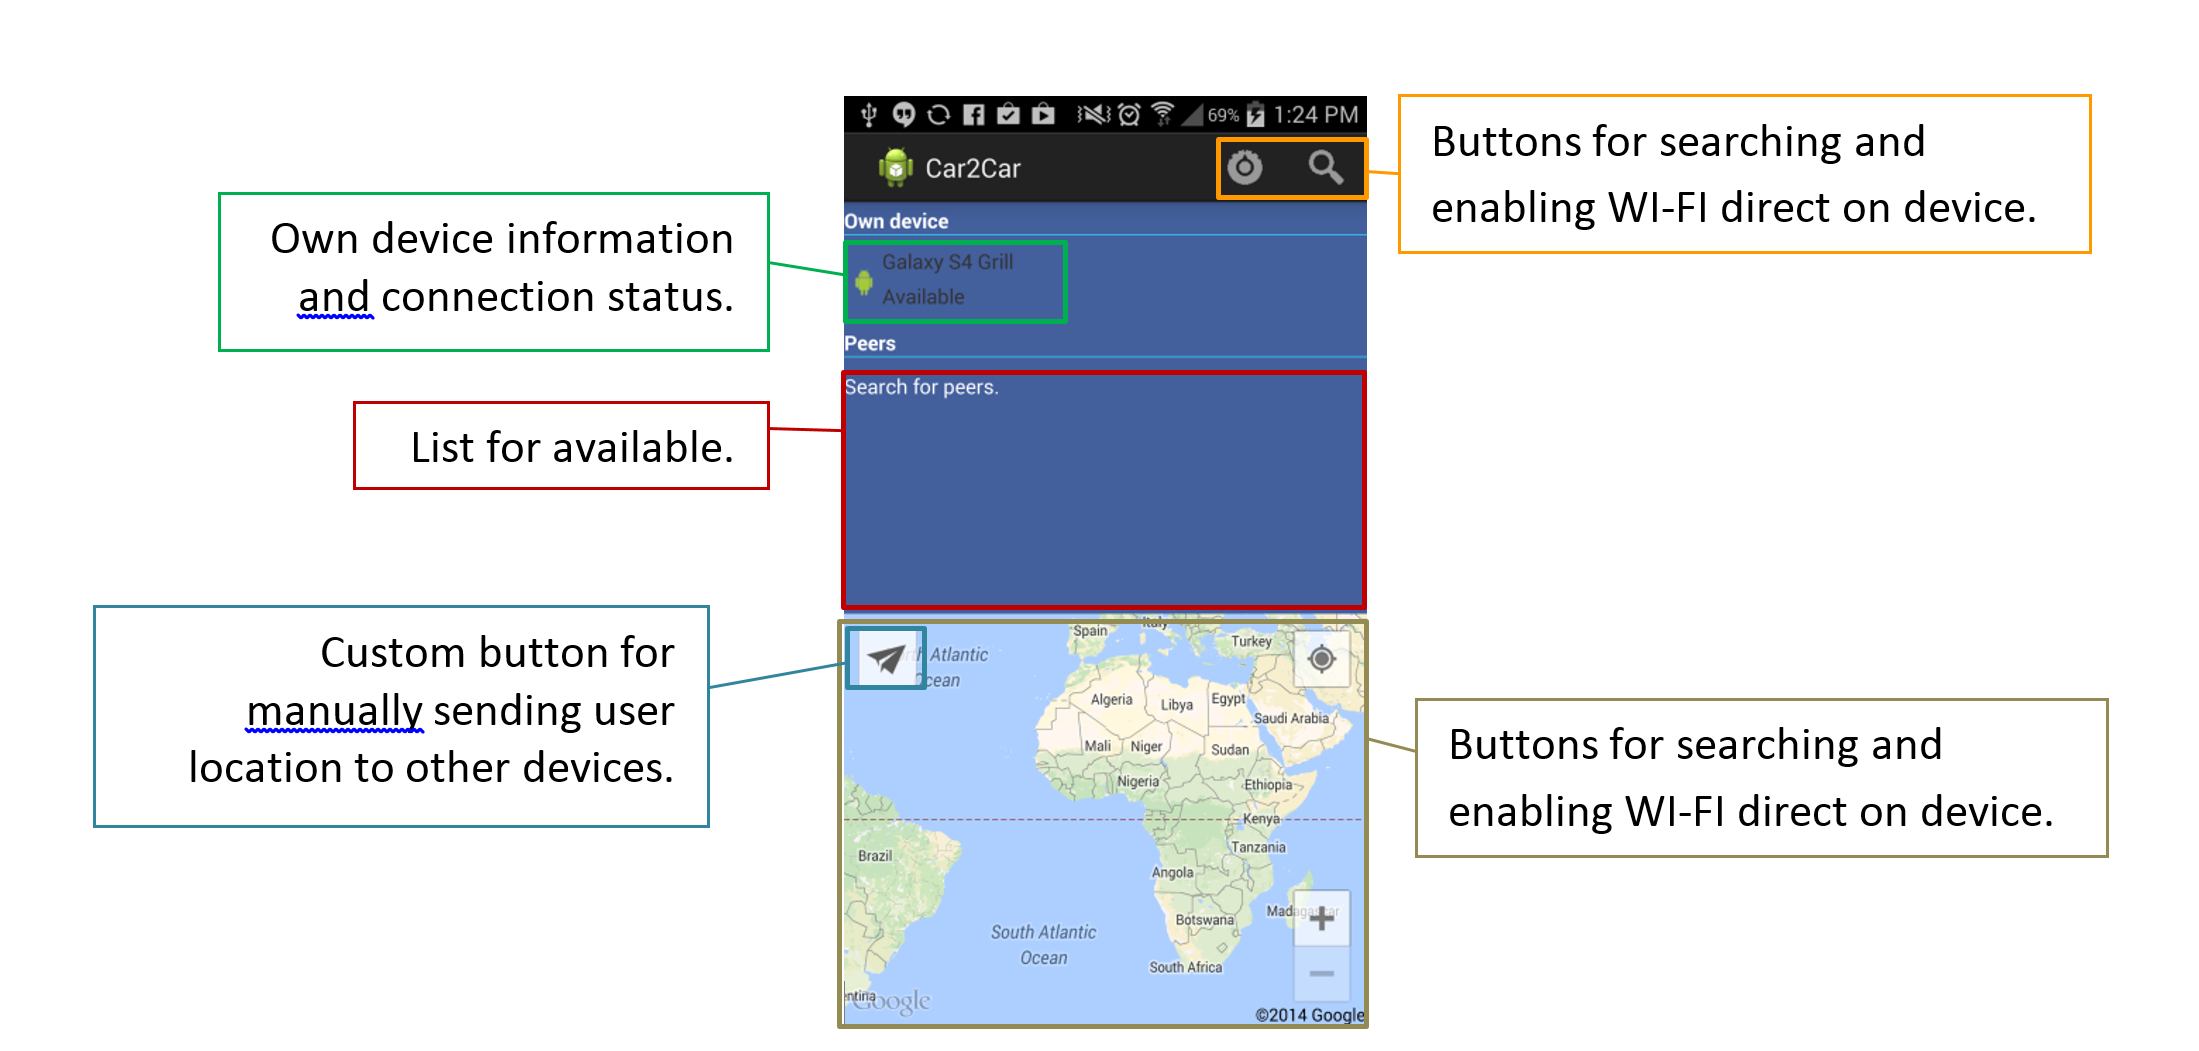
\includegraphics[width=0.9\textwidth]{images/androidScreen1.png}
	\caption{The figure shows the Android prototype application}
	\label{fig1}
\end{figure}

\noindent When the application is started it automatically begins to search for available peers. Additionally, the user can search manually by pressing the search button in top of the application. The application filters available peers per instance name, which means only other C2C peers are shown. If peers are available they appear immediately in the list view. A user can connect to other devices by clicking on the specific item in the list view. If the connection attempt was successful the invited device will get connection invitation which the user has to accept.  If the other user has accepted the invitation the two application shares their GPS location information. This means, every time the location of the device will change the current GPS information (Longitude and Latitude) will send to all connected peers. In some regions with weak GPS signals it could take several minutes until the application shares their GPS information with the other connected peers. The result of a successful connection is shown in the image below. The position of the other device is marked with a red google marker icon.


\begin{figure}[ht]
	\centering
  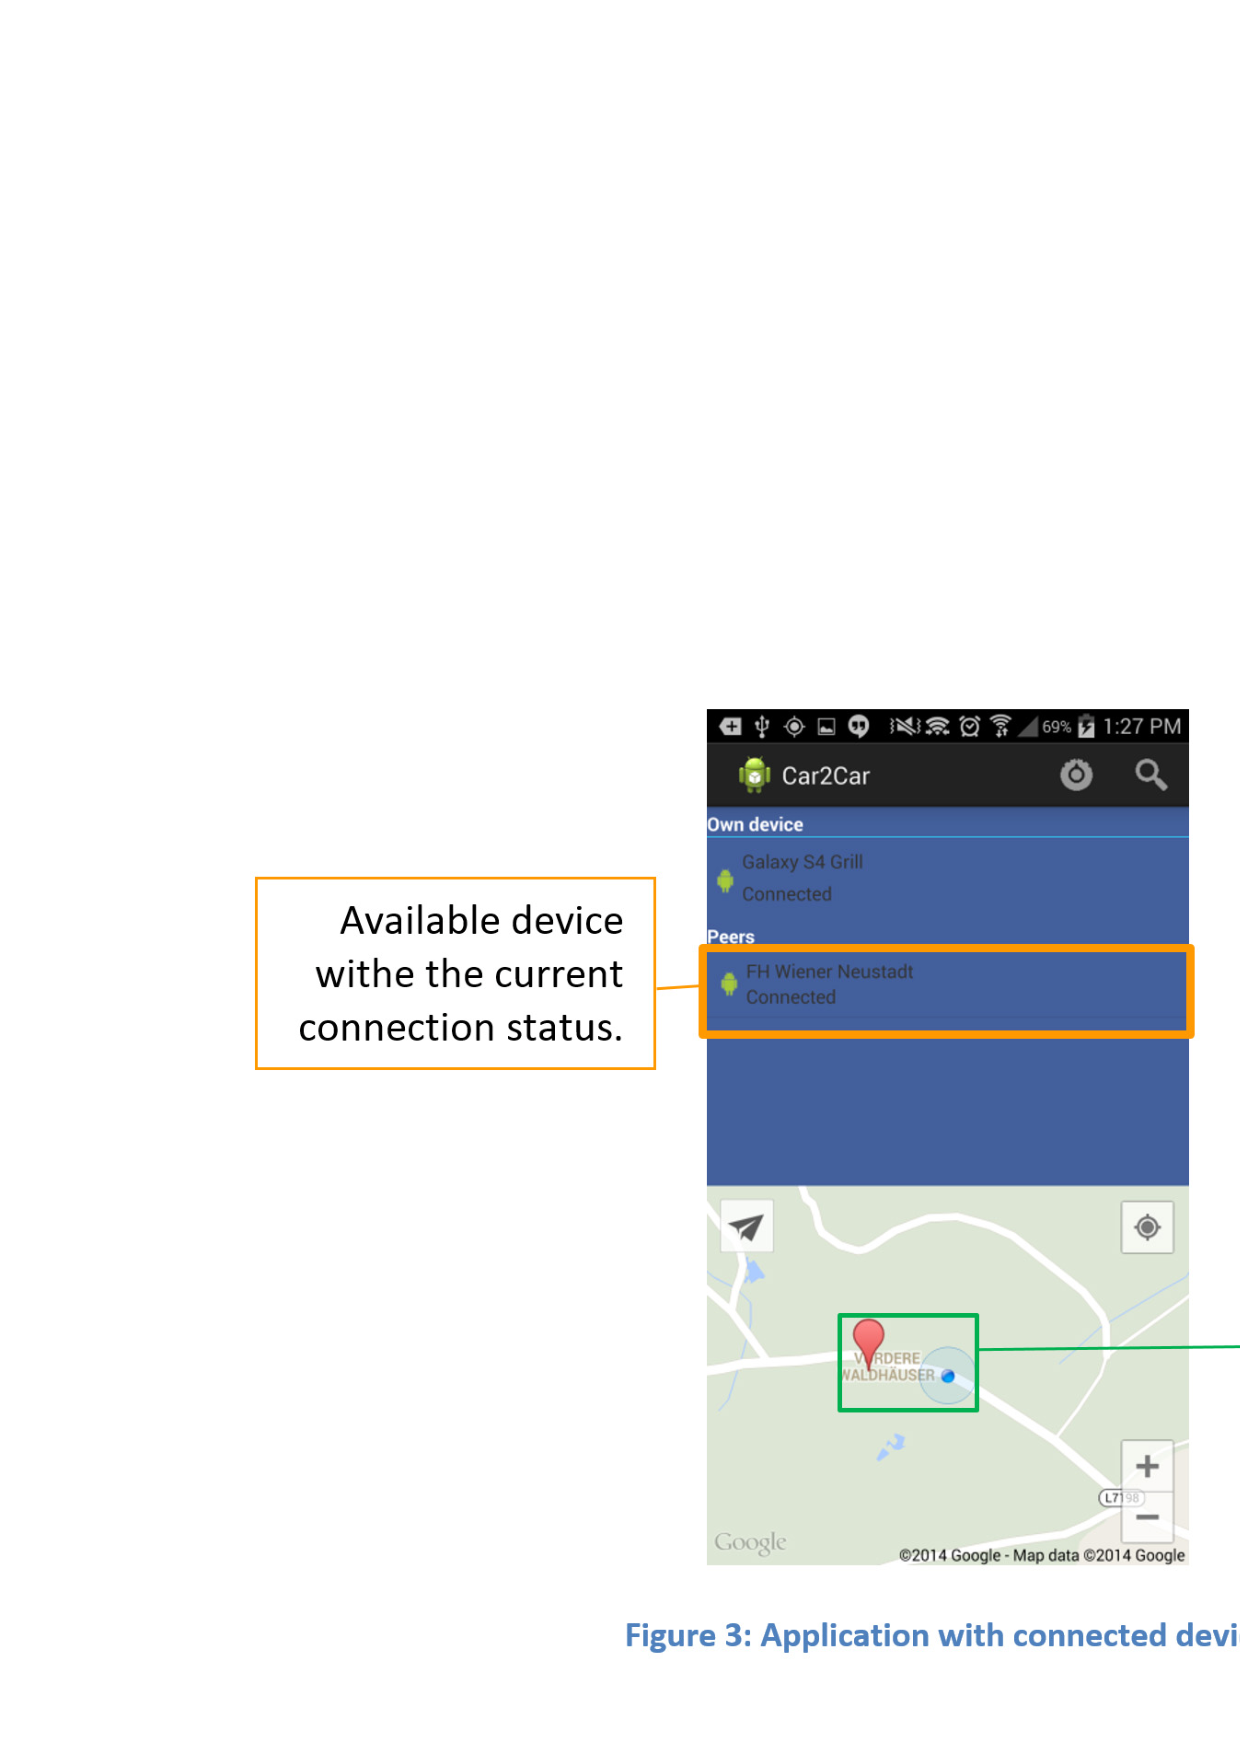
\includegraphics[width=0.9\textwidth]{images/androidScreen2.png}
	\caption{The figure shows the Android prototype application with a connected device}
	\label{fig1}
\end{figure}

\subsection*{Limitations and Problems}
\label{subsec:LimitationsProblems}
One of the biggest problems with Androids WI-FI P2P APIs, from the perspective of the C2C project, is the fact that every time a device wants to connect to your smartphone, it requires a confirmation from the user. Of course this had some security backgrounds and it make sense in other scenarios, but it is a major problem for using Android devices and this type of communication in the C2C project.  For obtaining detail information, like the current location or other important details, it is necessary that all devices are connected automatically to each other when they are in the same area. The image below shows an invitation message which shows up on every device which receives a connection request.
 
\begin{figure}[H]
	\centering
  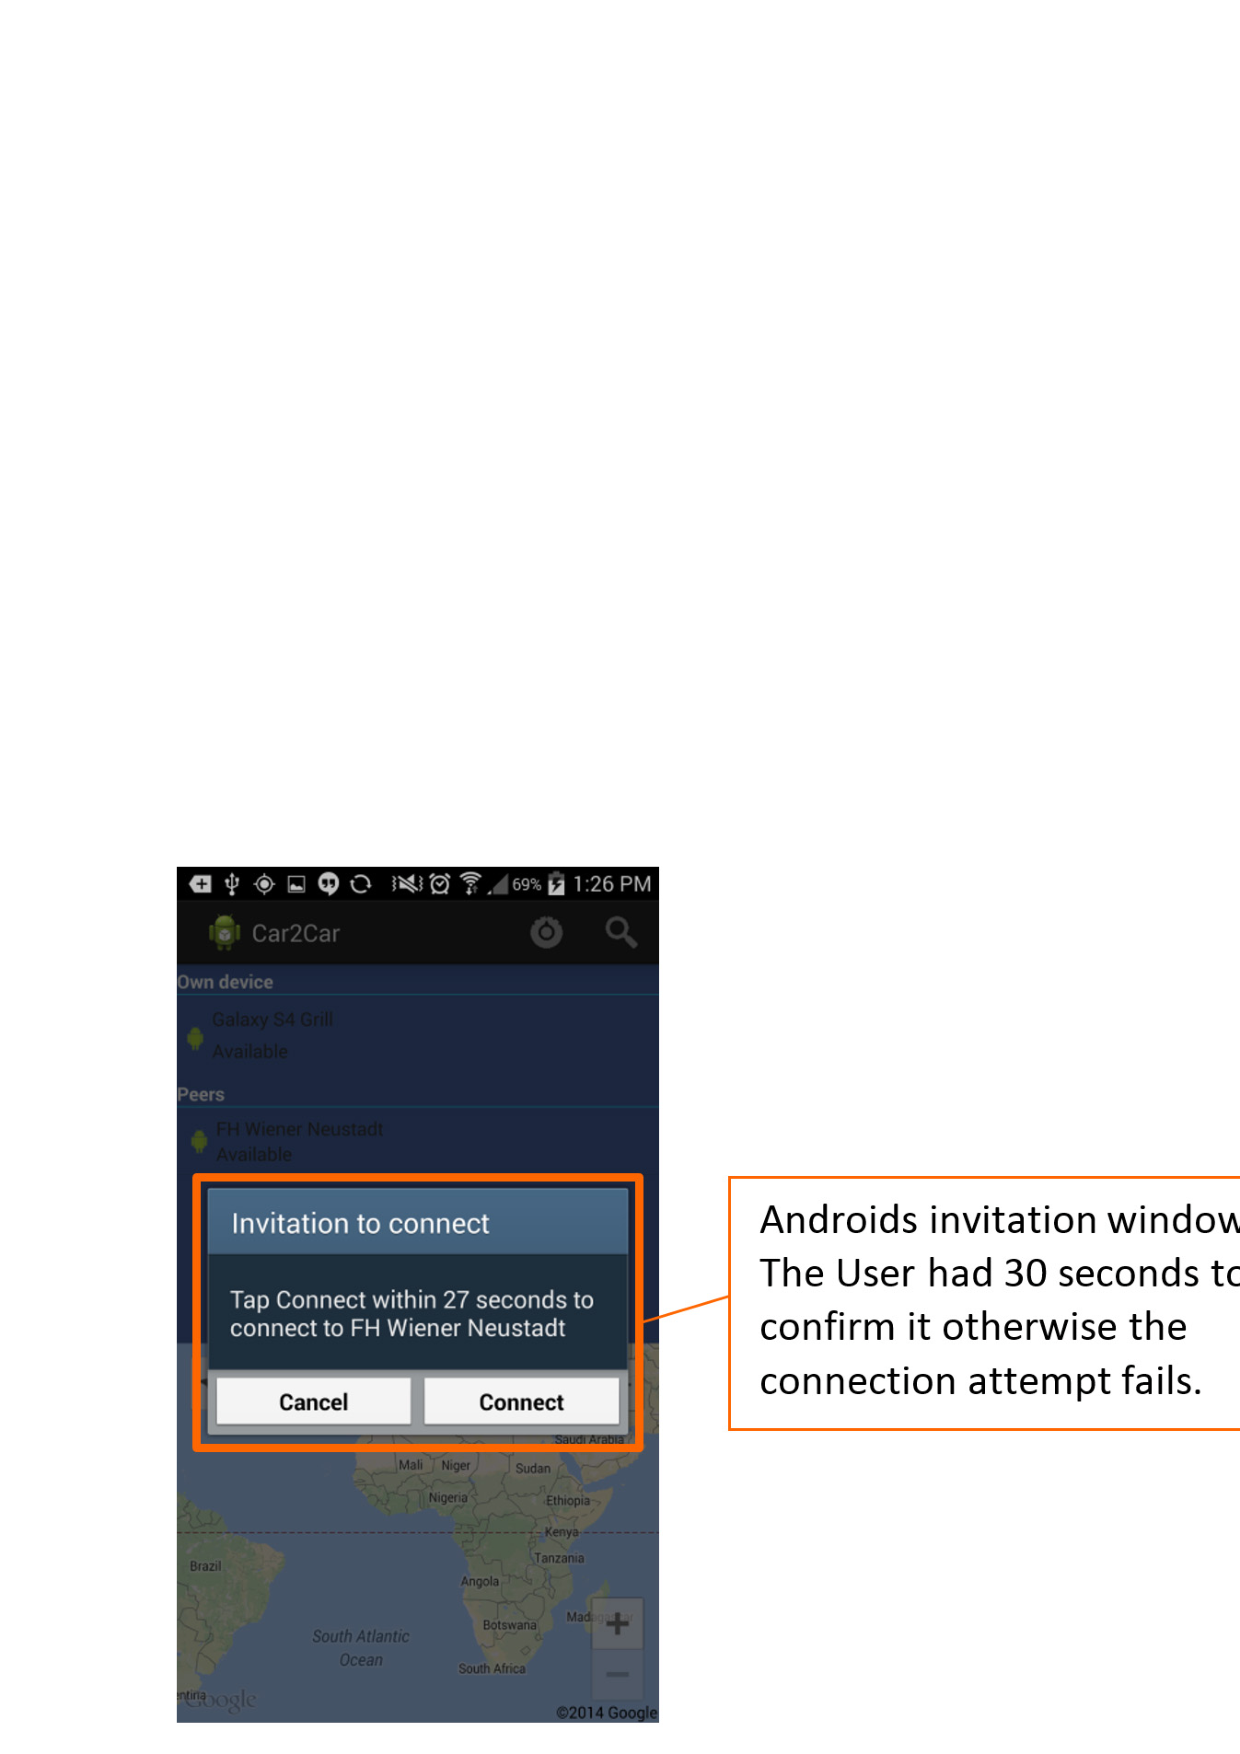
\includegraphics[width=0.9\textwidth]{images/androidScreen3.png}
	\caption{The figure shows the Android prototype application with a Wifi P2P connection request}
	\label{fig1}
\end{figure}

\noindent According to the WI-FI P2P documentation the range of the WI-FI P2P signal could be up to 500 meters. For the Android Car2Car prototype the test devices Samsung Galaxy S4 and Samsung Galaxy S2 Plus was used. It was not possible to confirm the range of 500 meters with the two devices. To test the maximal range of the signal, a few tests on a straight level road were carried out. It was determined that the signal at about 100-120 meters is lost. The tests were performed on foot and by car without any major differences. For a successful reconnect the distance between the devices was about 50-70 meters. The pictures below show the performed tests and describe their results.

\begin{figure}[H]
	\centering
  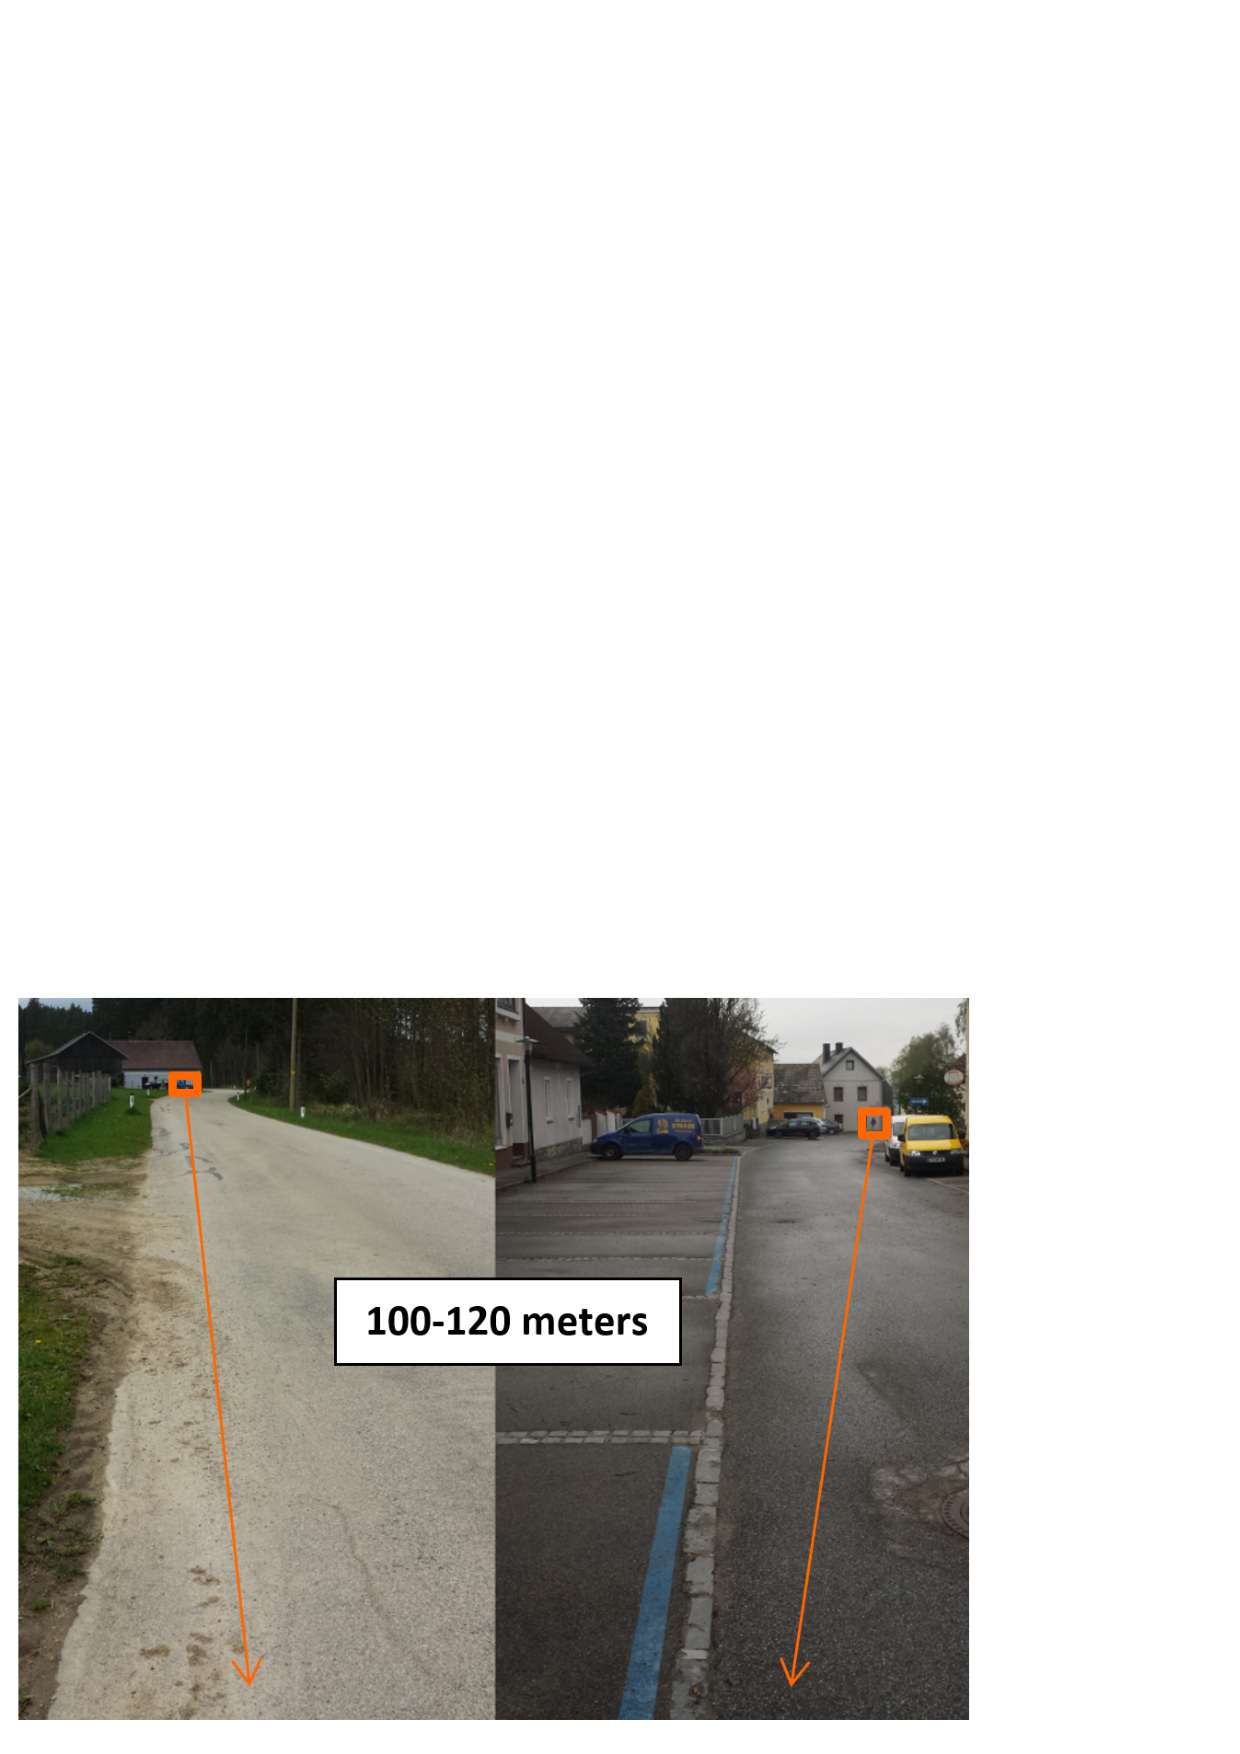
\includegraphics[width=0.9\textwidth]{images/androidScreen4.png}
	\caption{The figure shows the maximum range of the Wifi P2P signal}
	\label{fig1}
\end{figure}

\begin{figure}[H]
	\centering
  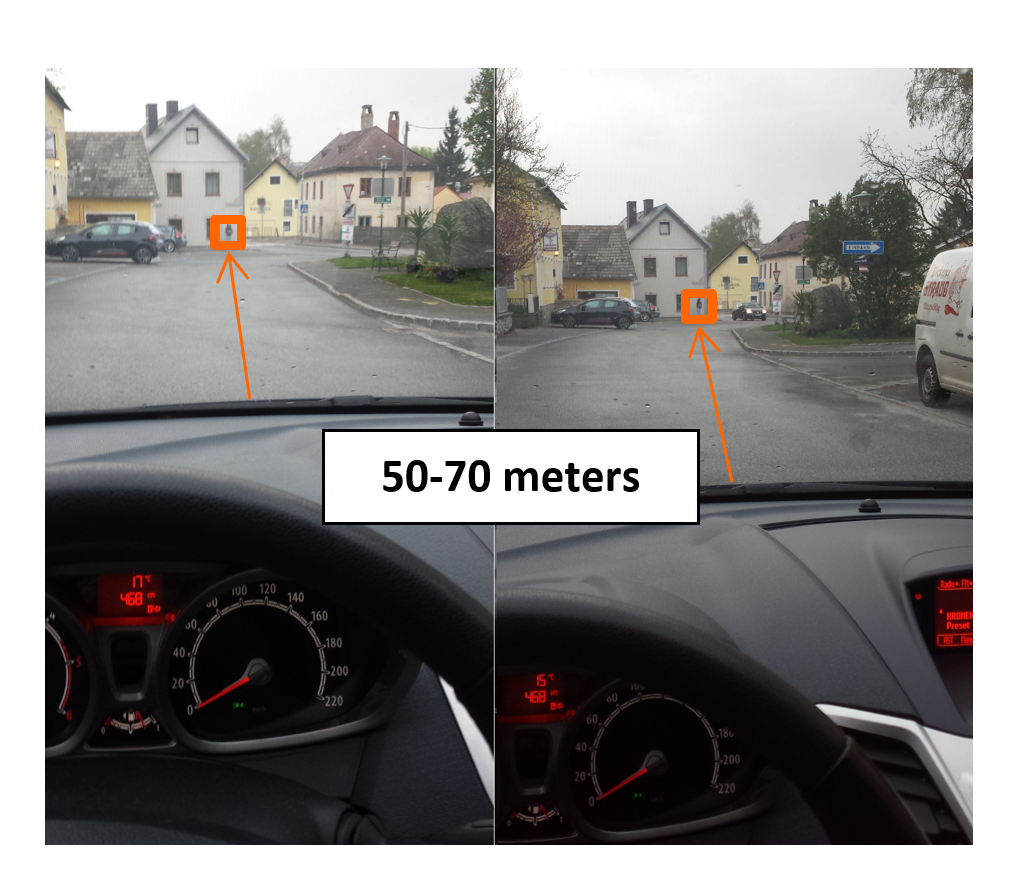
\includegraphics[width=0.9\textwidth]{images/androidScreen5.png}
	\caption{The figure shows the maximum distance for a successful reconnect}
	\label{fig1}
\end{figure}

\section{Rasberry Pi}
\label{sec:RasberryPi}

\section{Windows Phone}
\label{sec:WindowsPhone}
Microsoft included Wifi Direct in his new Windows Phone 8.1 SDK, but actually there is no good documentation or sample which describes the usage of Wifi Direct in a Windows Phone app.\\
The other option would be to use there own namespace which connects two phones directly to each other, but this requires Bluetooth and WIFI and the same app on both devices. Since this is not compatible with any other devices than Windows Phones this is not good solution. Furthermore are the devices limited to the Bluetooth range which is in fact not very long.